\chapter{Introduction}
\label{ch:intro}

\section{Motivation}

There are programming languages, like \texttt{Pascal}, \texttt{Ada} or \texttt{BASIC}, that distinguishes functions that do and do not
have return values,
the latter are known as procedures. C family languages do not. Pre-standardisation C language did not have \lstinline{void} functions,
instead an unspecified return value defaulted to \lstinline{int}. This resulted in functions declared with \lstinline{int} return value
not returning anything and the supposed return value was unused on purpose. One of its consequences was for example, that for a while if
you wrote a function, that was declared to return \lstinline{int} without the return value, the compiler did not act on it. When writing
code in C++ we often use functions from C, and a lot of standard library POSIX function behaves as a C function. % citation needed

\section{Problem Statement}

There are quite a few functions whose return value is often ignored, which could lead to potential bugs. Some examples:

\begin{itemize}
	\item POSIX \texttt{read}: returns the number of files read; this return value can also indicate errors with it being -1.
	\item POSIX \texttt{scanf}: returns the number of items in the argument list successfully filled; also indicates errors with EOF return.
	\item (cstdio) \texttt{std::remove}: return indicates success or error.
	\item (algorithm) \texttt{std::remove}: Does not remove. It returns an iterator, and we still need to use erase for all elements after this iterator.
	\item \texttt{std::remove\_if}: Same as remove.
	\item container specific \texttt{erase}: Returns an iterator to the next element after the removed. 
	\item container specific \texttt{insert}: Returns an iterator to the first of the new elements inserted.
\end{itemize}

Later the attribute \texttt{[[nodiscard]]} \cite{cppreferencenodiscard} was introduced to notify and give warnings to the user if the return value was unused in case
of a function
with this attribute, but in ask the compiler to give warnings on unchecked values, we would need permission to modify the library code.
In case of external source code such as POSIX, STL or any third party project, we will not have permission to do so.
We still need to notify the user on the cases where they do not check non-void return value. This brings us back to static analysis.

\section{Static analysis}

Static analysis is a method to analyse the source code of software projects without performing a real execution of the application.
It is widely used in industry to find bugs and code smells during development, to aid in the prevention of bad code that misbehaves in
production.
Among various methods, the most important techniques are the ones that are based on pattern matching on a syntactic representation of
the software project.

Clang-Tidy is a declarative, object oriented, strong typed static analysis rule collection that is built upon the LLVM Compiler
Infrastructure's C-family compiler, Clang.
It performs pattern matching on Clang's "Abstract Syntax Tree" (AST) representation, and generating diagnostics based on which analysis
modules, called "checks", the user turns on. We will address both the LLVM library and AST matchers in later chapters of the thesis.


\begin{figure}
    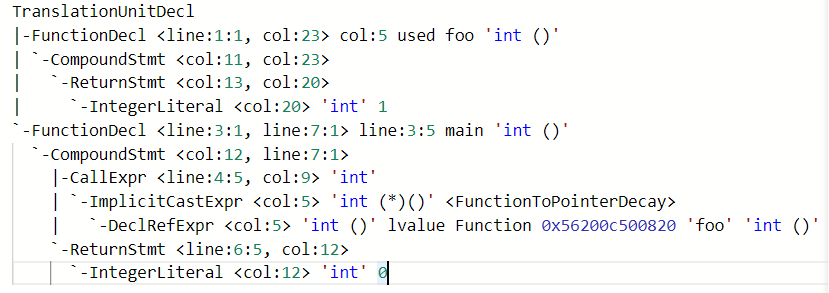
\includegraphics[width=\linewidth]{images/random_ast_example.png}
	\caption{An example of an Abstract Syntax Tree} % TODO maybe cite gotbolt?
\end{figure}

Let us imagine a checker, that keeps a statistics on how many times a return value of a non-\texttt{void} function is used, or otherwise known
as checked. This property is, as we previously stated important, because there exist a great amount of functions,
whose return value should be checked in most situations but remain unchecked in quite a lot.

\section{Infrastructure Limitations}

Unfortunately, for programming languages in the C family, such as C++, the concept of "separate translation" causes issues for static
analysis. As most static analysers are built upon compilers, and in C++, each compiler only sees the local information in the source file
(also known as the Translation Unit) it is to compile or analyse (as opposed to project-level knowledge), crucial details
might be hidden, which lowers, or in most cases, completely distorts the accuracy of the analysis.
This means that the way our infrastructure works, a checker like this would be of very limited use.

A function can obviously exist outside of the translation unit of its declaration. If such analysis with our imagined checker is done
separately on each translation unit, it is easy to see how that can affect the outcome. A function might be called 100 times and 
checked 95 times through. We would want to give warnings for the unchecked 5\% of those calls, but if, for example, these are in a 
separate translation unit, then the analysis would return with 0 checks out of 5 calls. We would not want to give warnings to a
function that is unchecked in all 100\% of its calls. The detail of the statistics, that it was only unchecked in 5\% is lost,
unless we use project level knowledge during our analysis. Consider another example, with code:

\begin{lstlisting}[language={C++},caption={An example of the infrastructure's limitations},label={lst:motivation example}]
// First translation unit
std::vector<int> c{0, 1, 2, 3, 4, 5, 6, 7, 8, 9, 11, 13, 15};

auto iter = c.erase(c.begin());
iter = c.erase(iter + 2, iter + 5);

for (std::vector<int>::iterator it = c.begin(); it != c.end(); ) {
    if (*it % 2 == 0) {
        it = c.erase(it);
    } else {
        ++it;
    }
}

// Second translation unit

std::vector<int> c{0, 1, 2, 3, 4};
for (std::vector<int>::iterator it = c.begin(); it != c.end(); ++it) {
    if (*it % 2 == 0) {
        c.erase(it);
    }
}
\end{lstlisting}

Here, with separate analysis, we would get 100\% checked in the first TU and 0\% in the second one. With project level knowledge, however we
would get 57\%. We used erase without a care towards its return value, and this could lead to potential bugs, but without the project
level knowledge, however we can not diagnose it.

The separate analysis could also create false positive results. Imagine we have a function whose return value we could use but it is mostly
optional. We could give our checker a treshold of percentage, to only diagnose unused values if we usually use them in most cases. Again, this
means that with different translation units, we do not know how many times we actually ignored the value and can not use our treshold properly.
This leads to false positive diagnosis.

Unfortunately, the current versions of Clang-Tidy checks can only access what is visible to the compiler, which is a local information.
Several classes of security issues and bad coding patterns might be diagnosed if the implemented checks would be capable of creating 
percompilation knowledge, and reusing the full knowledge about the project during diagnosis.
The work of the thesis is to enhance Clang-Tidy on the infrastructure level to support multi-pass analyses in a generic manner, by 
utilizing the ideas similar to that of MapReduce \cite{mapreduce}.

This is achieved by allowing individual checks to store check-specific data on a thread-safe location.
A subsequent execution of the analysis will be able to do the pattern matching fine-tuned with the data stored in the previous step also
available.
To prove the usability of the solution, a new safety and security related check, currently not provided by Clang-Tidy, will be developed
utilizing the new infrastructure created in this work.
In the end, the results of the thesis will allow the international community behind LLVM to develop and make available a wider potential of
checks, as we are planning to upstream the entire project into LLVM. \cite{upstream1} \cite{upstream2} \cite{upstream3}

\section{Related Works}

The topic of cross translation unit analysis shares other different solutions and implementations as well, one great example is
Clang CTU \cite{clangCTU}.
As previously stated, the infrastructure enhancement follows the philosophy of MapReduce \cite{mapreduce}.
There exists a static analysis rule in Coverity Scan static analysis tool, that is similar to our checker \cite{coverity}.


\section{Thesis layout}

After the Introduction, in \cref{ch:user}, the User Guide will have instructions on how to download, compile and set up the static analysis tool, and
how to run it on a C++ project. In \cref{ch:impl}, the Developer Guide will explain how the checker, and the infrastructure itself works, in detail.
